\documentclass[10pt,a4paper]{article}
\usepackage[utf8]{inputenc}
\usepackage[english]{babel}
\usepackage{amsmath}
\usepackage{amsfonts}
\usepackage{amssymb}
\usepackage{graphicx}
\usepackage{grffile}
\usepackage{float}
\usepackage{hyperref}
\usepackage[left=2cm,right=2cm,top=2cm,bottom=2cm]{geometry}
\usepackage{listings}
\usepackage{verbatim}
\lstset{basicstyle=\ttfamily,
  showstringspaces=false,
  commentstyle=\color{red},
  keywordstyle=\color{blue}
}
\author{Julia Desmazes}
\title{Lab1 Rasbian RT}
\begin{document}
\section{Latency test}
\subsection{Supported schedualing policies}
\subsection{Cyclictest}
%). The measuring threads are woken up periodically with a defined interval by an expiring timer (cyclic alarm). Subsequently, the difference between the programmed and the effective wake-up time is calculated and handed over to the master thread via shared memory. The master thread tracks the latency values and prints the minimum, maximum and average for the latency once the number of iterations specified is completed. 
Cyclictest is a programme included in the rt\_test suite to measure the latency of an particular environement. It creats a defined number of threads that it wakes up at set intervals and then measures the latency between the moment the thread was expected to wake-up and the actual time the action took place.\\
Reading the \emph{-h} guide we can learn that \emph{-t} allows us to set the number of threads we wish to create and \emph{-p} sets the priority. 
\paragraph{threads \emph{-t}}
More precisly if no parameter is give the number of threads will be equal to the number of cpus and the execution of thows threads will be ballanced equlay\footnote{under the best possible conditions} between they s different cpu's. As we are currently on a 4 cpu system if we wish to create 4 threads leaving it to the default option would be correct. But if we didn't specify the \emph{-t} option then only 1 thread would have been created.
\begin{lstlisting}[language=bash,caption={cyclictest -h}]
-t       --threads         one thread per available processor
-t [NUM] --threads=NUM     number of threads:
without NUM, threads = max_cpus
without -t default = 1
\end{lstlisting}
\paragraph{priorities \emph{-p}}
%By default threads are squeduqled with SCHED_FIFO under cyclictest
In linux priority ranges are fixed by the schedualing algorythme used. by default cyclictest runs SCHED\_FIFO\footnote{See patch for fix \url{https://www.spinics.net/lists/linux-rt-users/msg05449.html}} and it's priorities will range from 0 to 99. Here priorities are reversed with 99 beeing the highest priority and 0 the lowest.
\begin{lstlisting}[language=bash,caption={cyclictest -h}]
-p PRIO  --prio=PRIO       priority of highest prio thread
\end{lstlisting}
\subsection{Test}
\paragraph{SHED\_FIFO}
\emph{Missing shed\_other !!}
\begin{figure}[H]
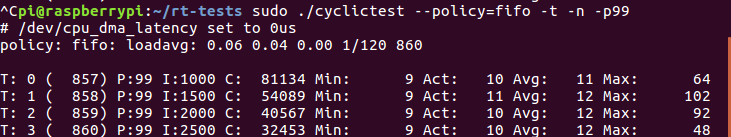
\includegraphics[width=16cm]{Voluntary-Fifo-WithoutHackbench.png}
\caption{SHED\_FIFO volontary}
\end{figure}
\begin{figure}[H]
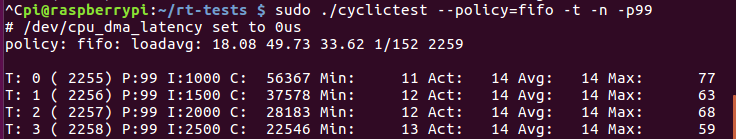
\includegraphics[width=16cm]{Preempt-Fifo-WithoutHackbench.png}
\caption{SHED\_FIFO preempt-rl}
\end{figure}
\paragraph{SHED\_RR}
\begin{figure}[h]
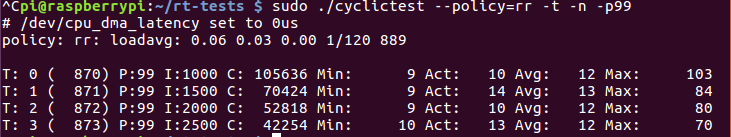
\includegraphics[width=16cm]{Voluntary-RR-WithoutHackbench.png}
\caption{SHED\_RR volontary}
\end{figure}
\begin{figure}[H]
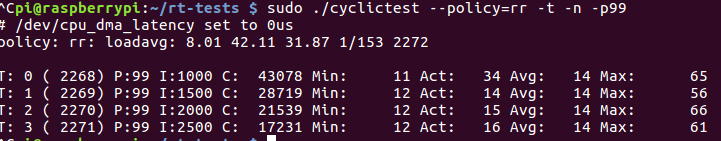
\includegraphics[width=16cm]{Preempt-RR-WithoutHackbench.png}
\caption{SHED\_RR preempt-rl}
\end{figure}
%Todo need shed other to conclude
\subsection{Cyclictest + Hackbench}
\subsubsection{Hackbench under SHED\_OTHER and priority 20}
\begin{figure}[H]
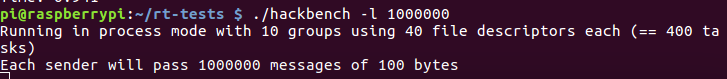
\includegraphics[width=16cm]{Volontary-other-Hackbench-p20.png}
\caption{Hackbench under SHED\_OTHER and priority 20}
\end{figure}
\paragraph{Volontary}
\begin{figure}[H]
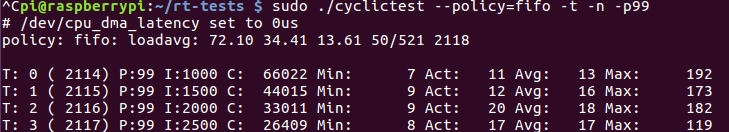
\includegraphics[width=16cm]{Volontary-Fifo-WithHackbench1.png}
\caption{Volontary fifo with hackbench}
\end{figure}
\begin{figure}[H]
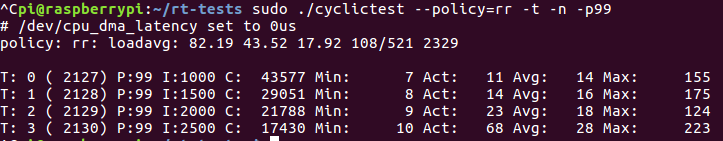
\includegraphics[width=16cm]{Volontary-Rr-WithHackbench1.png}
\caption{Volontary rr with hackbench}
\end{figure}
\paragraph{Preempt-rt}
\begin{figure}[H]
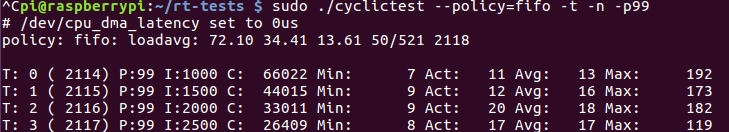
\includegraphics[width=16cm]{Volontary-Fifo-WithHackbench1.png}
\caption{Volontary fifo with hackbench}
\end{figure}
\begin{figure}[H]
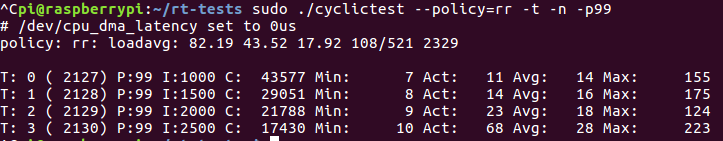
\includegraphics[width=16cm]{Volontary-Rr-WithHackbench1.png}
\caption{Volontary rr with hackbench}
\end{figure}
\emph{Missing tests on preempt-rt kernel}
\subsubsection{Hackbench under RT scheduling policies and priority 49}
\paragraph{SHED\_FIFO}
\begin{figure}[H]
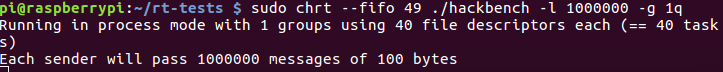
\includegraphics[width=16cm]{Hackbench2.png}
\caption{Hackbench with shed\_fifo and priority 49}
\end{figure}
\begin{figure}[H]
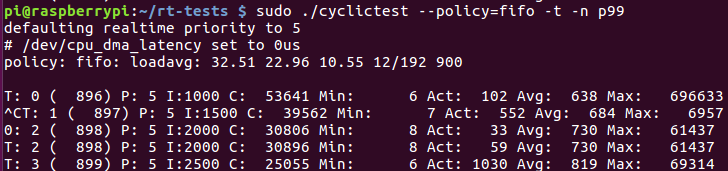
\includegraphics[width=16cm]{Preempt-Fifo-WithHackbench2.png}
\caption{Preempt-rt with fifo}
\end{figure}
\begin{figure}[H]
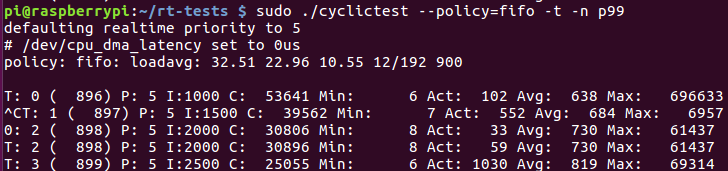
\includegraphics[width=16cm]{Preempt-Fifo-WithHackbench2.png}
\caption{Preempt-rt with fifo}
\end{figure}
\paragraph{SHED\_RR}
\emph{Missing hackbench with sched -rr 49 and accompaning tests}
%todo alsk the teatcher if we sould have done this test on the volontary if so missing even more screenshots
Can't finish missing screanshots
\section{ADA concurrent programs}
\subsection{Program 1}
\paragraph{code}
\begin{figure}[H]
\begin{center}
\verbatiminput{main.adb}
\caption{Program 1}
\end{center}

\end{figure}

\paragraph{Observations}
The A,B,C,D are printed in order throwout the execution with there not beeing any apparent modification of that ordered sequence.
\subsection{Program 2}
\paragraph{code}
\begin{figure}[H]
\begin{center}
\verbatiminput{main2.adb}
\caption{Program 2}
\end{center}

\paragraph{Observations}
%Todo recall the main diffrences between the two packages and constructs
In this test we can observe that even thow both treads are confirured to sleep for the same 100ms time interval they eventually end up off sync. We can attribute this to the diffrence between the way time is treated in the \emph{delay} and \emph{delay until}.
%todo finish later 
\end{document}